\section{Projekt aplikacji} 
Rozplanowanie działania aplikacji pozwala na przemyślaną implementację wszystkich funkcji. Przed stworzeniem aplikacji należy dokładnie zastanowić się nad najważniejszymi wymaganiami funkcjonalnymi i niefunkcjonalnymi, przypadkami użycia aplikacji, a także zaprojektować model danych. Przydatne jest także rozpisanie przykładowych scenariuszy, które mogą wystąpić przy korzystaniu z aplikacji przez użytkownika. Wcześniejsze zaprojektowanie przykładowych interfejsów użytkownika pomaga dostosować wygląd systemu do potrzeb grupy docelowej. Poniższy rozdział skupia się na przedstawieniu projektu aplikacji zawierający wszystkie wcześniej wymienione elementy.
    \subsection{Wymagania funkcjonalne}
    \noindent
    \textbf{Administrator}
    \begin{enumerate}
        \item Zarządzanie trasami dostępnymi w systemie
        \begin{enumerate}
            \item Dodawanie nowych tras (jeśli nowe zostały wyznaczone).
            \item Rozbudowa bazy tras o nowe regiony.
            \item Aktualizacja istniejących w systemie szlaków i ich opisów.
            \item Usuwanie szlaków, które są tymczasowo wyłączone z użycia przez TPN (np. \\w celu modernizacji).
        \end{enumerate}
        \item Obsługa powiadomień
        \begin{enumerate}
            \item Wysyłanie powiadomień ogólnosystemowych do wszystkich użytkowników.
            \item Przekazywanie komunikatów wychodzących odgórnie o możliwym zagrożeniu (np. zagrożenie lawinowe, burze ogłaszane przez TPN/GOPR).
            \item Wysyłanie powiadomień do użytkowników w obrębie konkretnego regionu o miejscowym zagrożeniu bądź utrudnieniach.
            \item Akceptacja powiadomień przesyłanych przez użytkowników o zgłoszonych incydentach na danej trasie.
        \end{enumerate}
    \end{enumerate}
    \textbf{Użytkownik}
    \begin{enumerate}
        \item Planowanie trasy
        \begin{enumerate}
            \item Zaznaczanie na mapie wybranego szlaku.
            \item Pobieranie map na urządzenie celem korzystania z aplikacji w trybie offline.
            \item Dodawanie pobocznych, wyznaczonych w aplikacji szlaków do głównej trasy.
            \item Edytowanie trasy w dowolnym momencie.
            \item Dodawanie punktów postojowych
        \end{enumerate}
        \item Pomoc
        \begin{enumerate}
            \item Dostęp do numerów alarmowych i lokalnych numerów ratunkowych (GOPR itp.)
            \item Wybieranie numeru z poziomu aplikacji i dzwonienie bez konieczności kopiowania numeru.
        \end{enumerate}
        \item Zgłaszanie zagrożeń
        \begin{enumerate}
            \item Wybieranie zagrożeń z dostępnych domyślnych opcji.
            \item Zgłaszanie innego typu zagrożenia z pełnym jego opisem.
            \item Wybranie możliwego regionu, na którym dane zagrożenie może występować.
            \item Wypełnienie zgłoszenia możliwe w trybie offline, wysłanie zgłoszenia do administratora tylko po połączeniu z internetem.
        \end{enumerate}
        \item Przegląd historii wędrówek
        \begin{enumerate}
            \item Generowanie raportu z wybranego okresu.
            \item Filtrowanie przebytych tras.
        \end{enumerate}
        \item Nawigacja
        \begin{enumerate}
            \item Korzystanie z map w trybie offline.
            \item Naprowadzanie na szlak w wypadku zejścia z niego.
            \item Otrzymywanie powiadomień o zagrożeniach na podstawie obecnej lokalizacji (tryb online)
        \end{enumerate}
        \item Krokomierz
        \begin{enumerate}
            \item Obliczanie spalonych kalorii na podstawie aktywności zarejestrowanej przez krokomierz.
            \item Generowanie podsumowań jednodniowych, tygodniowych lub z wybranego okresu.
        \end{enumerate}
        \item Logowanie
        \begin{enumerate}
            \item Zakładanie konta.
            \item Usuwanie konta.
            \item Edytowanie danych.
        \end{enumerate}
    \end{enumerate}

    \subsection{Wymagania niefunkcjonalne}
    \begin{enumerate}
        \item System zbudowany na urządzenia mobilne z systemem Android w wersji 7.0 lub wyższej.
        \item System wykorzystuje moduł GPS celem nawigacji po wyznaczonych szlakach.
        \item System wykorzystuje krokomierz (jeśli urządzenie takowy posiada) celem liczenia kroków i spalonych przez użytkownika kalorii.
        \item System powinien zapewniać bezpieczeństwo danych użytkowników, zwłaszcza szczególnie wrażliwych informacji takich jak dane osobowe.
        \item System powinien posiadać zrozumiały interfejs użytkownika w celu łatwego korzystania z niego.
        \item System powinien umożliwiać monitorowanie jego działania w celu ułatwienia rozwiązywania problemów.
        \item Hasła użytkowników powinny być szyfrowane.
    \end{enumerate}

    \subsection{Diagramy przypadków użycia}
    Diagramy przypadków użycia pozwalają w prosty sposób zwizualizować dostępne dla poszczególnych ról funkcje oraz ich przebiegi. Pozwalają także na uwzględnienie wyjątków i ewentualnych problemów, jakie użytkownik może napotkać podczas korzystania z systemu.

    Poniższe diagramy prezentują poszczególne funkcje aplikacji oferowane poszczególnym rolom użytkowników opracowane na podstawie określonych wcześniej wymagań funkcjonalnych. Zestaw funkcji jest inny dla każdego aktora. Użytkownik ma możliwość zarządzania swoim kontem, przejrzenia wędrówek, wezwanie pomocy oraz zaplanowania trasy z opcją punktów postojowych. Administrator posiada mniej funkcji, w ich skład wchodzą obsługa powiadomień oraz zarządzanie bazą szlaków.
    \setlength{\fboxrule}{0.5pt}
    \begin{figure}[H]
        \centering
        \fbox{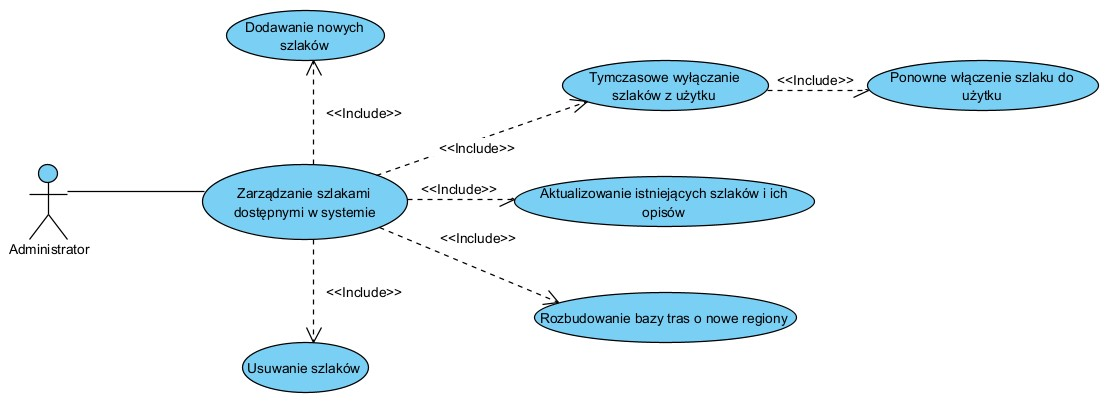
\includegraphics[width=\linewidth]{img/diagramy/UCD/UCDszlaki.jpg}}
        \caption{Diagram przypadku użycia: zarządzanie szlakami przez administratora.}
        \label{ucd:szlaki}
    \end{figure}
    Funkcja zarządzania szlakami przez administratora (rys. \ref{ucd:szlaki}) składa się z kilku pomocniczych funkcji. Są to między innymi: tymczasowe wyłączanie z użytku (np. na potrzebę modernizacji szlaku bądź usunięcia z niego powalonych drzew), ponowne jego włączenie do użytku, dodawanie nowych szlaków, usuwanie szlaków, aktualizacja przebiegu istniejących szlaków oraz rozbudowanie bazy tras o nowe regiony i kolejne pasma górskie.

    \setlength{\fboxrule}{0.5pt}
    \begin{figure}[H]
        \centering
        \fbox{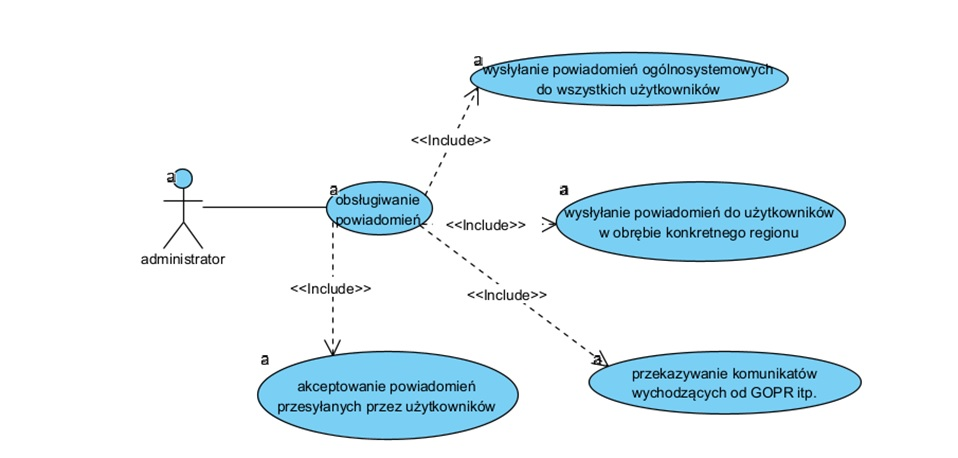
\includegraphics[width=\linewidth]{img/diagramy/UCD/UCDpowiadomieniaAdmin.jpg}}
        \caption{Diagram przypadku użycia: obsługa powiadomień po stronie administratora.}
        \label{ucd:powiadomienia}
    \end{figure}
    
    Funkcja obsługi powiadomień (rys. \ref{ucd:powiadomienia}) dostępna dla administratora pozwala na wysyłanie powiadomień do użytkowników w obrębie konkretnego regionu, wysyłanie powiadomień ogólnosystemowych do wszystkich użytkowników, przekazywanie komunikatów wychodzących od GOPR oraz akceptowanie zgłoszonych zagrożeń przesłanych przez użytkowników.

    \setlength{\fboxrule}{0.5pt}
    \begin{figure}[H]
        \centering
        \fbox{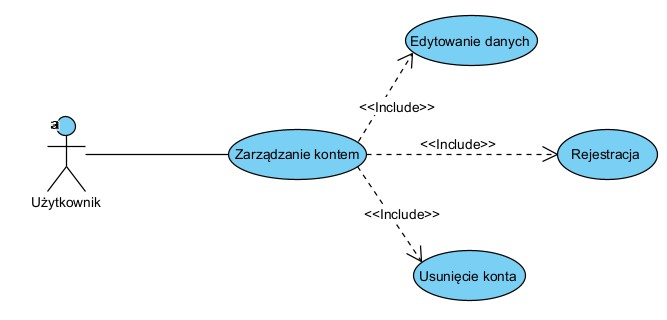
\includegraphics[width=\linewidth]{img/diagramy/UC/UCkonto.jpg}}
        \caption{Diagram przypadku użycia: zarządzanie kontem.}
        \label{ucd:konto}
    \end{figure}
    Zarządzanie kontem (rys. \ref{ucd:konto}) leży w całości po stronie użytkownika - wędrówkowicza. Powierzono mu takie funkcje jak: rejestracja, edytowanie danych przypisanych do konta oraz usunięcie konta.

    \setlength{\fboxrule}{0.5pt}
    \begin{figure}[H]
        \centering
        \fbox{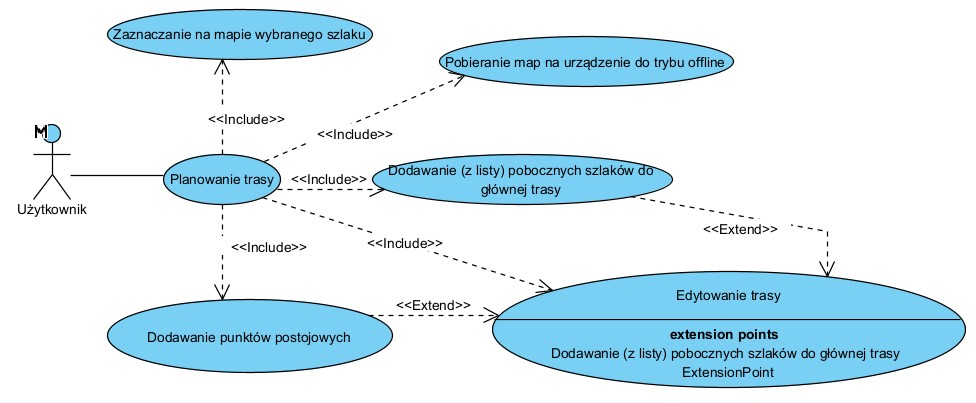
\includegraphics[width=\linewidth]{img/diagramy/UC/UCplan.jpg}}
        \caption{Diagram przypadku użycia: planowanie trasy przez użytkownika.}
        \label{ucd:planowanie}
    \end{figure}
    Planowanie trasy (rys. \ref{ucd:planowanie}) jest procesem umożliwiającym podróżującemu na wybranie proponowanych mu szlaków, aby przejść z jednego miejsca w drugie. Na ten proces składają się funkcje takie jak: zaznaczanie na mapie wybranego szlaku, dodawanie z listy przylegających szlaków do głównej trasy, dodawanie punktów postojowych,

    \setlength{\fboxrule}{0.5pt}
    \begin{figure}[H]
        \centering
        \fbox{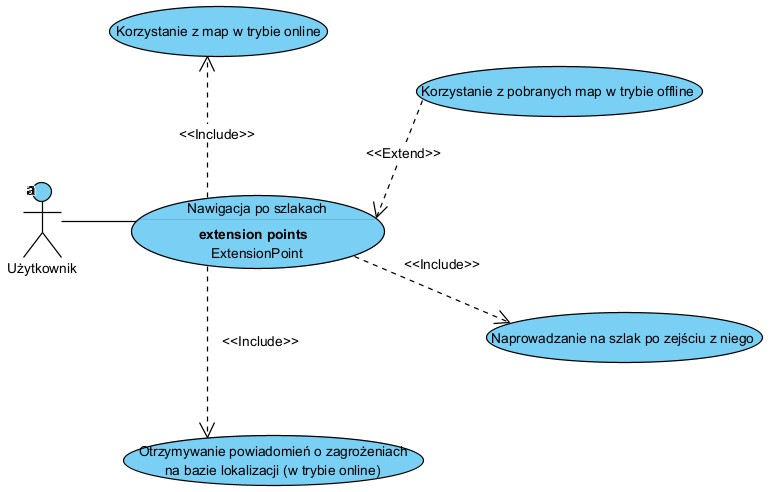
\includegraphics[width=\linewidth]{img/diagramy/UC/UCnawigacja.jpg}}
        \caption{Diagram przypadku użycia: nawigacja}
        \label{ucd:nawigacja}
    \end{figure}
    Nawigacja po szlakach górskich (rys. \ref{ucd:nawigacja}) jest głównym zadaniem aplikacji. Poprawne jej funkcjonowanie gwarantują takie elementy, jak: korzystanie z map w trybie online, otrzymywanie powiadomień o zagrożeniach bądź utrudnieniach na trasie, pobieranie map i korzystanie z nich w trybie offline oraz naprowadzanie na szlak po zejściu z niego.

    \setlength{\fboxrule}{0.5pt}
    \begin{figure}[H]
        \centering
        \fbox{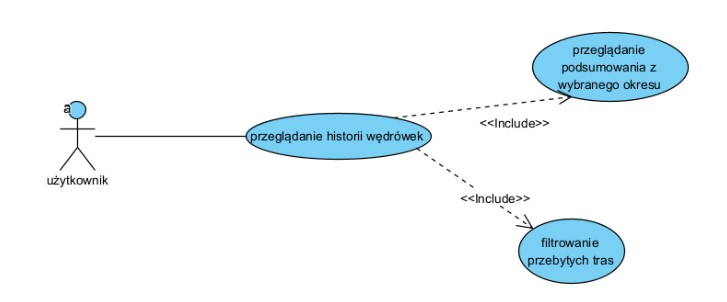
\includegraphics[width=\linewidth]{img/diagramy/UCD/UCDhistoria.jpg}}
        \caption{Diagram przypadku użycia: historia przebytych tras.}
        \label{ucd:historia}
    \end{figure}
    Przeglądanie historii przebytych tras przez danego użytkownika (rys. \ref{ucd:historia}) pozwala na kontrolowanie przebiegu swoich wędrówek. Dodatkową opcją tej funkcji jest generowanie raportów za ustalony okres, co ułatwia szybki powrót do swoich wypraw.

    \setlength{\fboxrule}{0.5pt}
    \begin{figure}[H]
        \centering
        \fbox{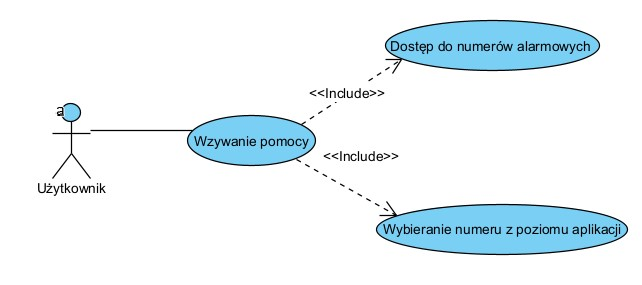
\includegraphics[width=\linewidth]{img/diagramy/UC/UCpomoc.jpg}}
        \caption{Diagram przypadku użycia: wzywanie pomocy.}
        \label{ucd:pomoc}
    \end{figure}
    Wzywanie pomocy na szlaku (rys. \ref{ucd:pomoc}) jest niezwykle istotną funkcją. Nie wszyscy turyści znają numery alarmowe, w tym numer GOPRu, często przed wyjściem na szlak zapominają ich zapisać. W związku z tym aplikacja udostępnia im opcję skopiowania numerów oraz bezpośredniego wybierania ich z poziomu aplikacji.

    \setlength{\fboxrule}{0.5pt}
    \begin{figure}[H]
        \centering
        \fbox{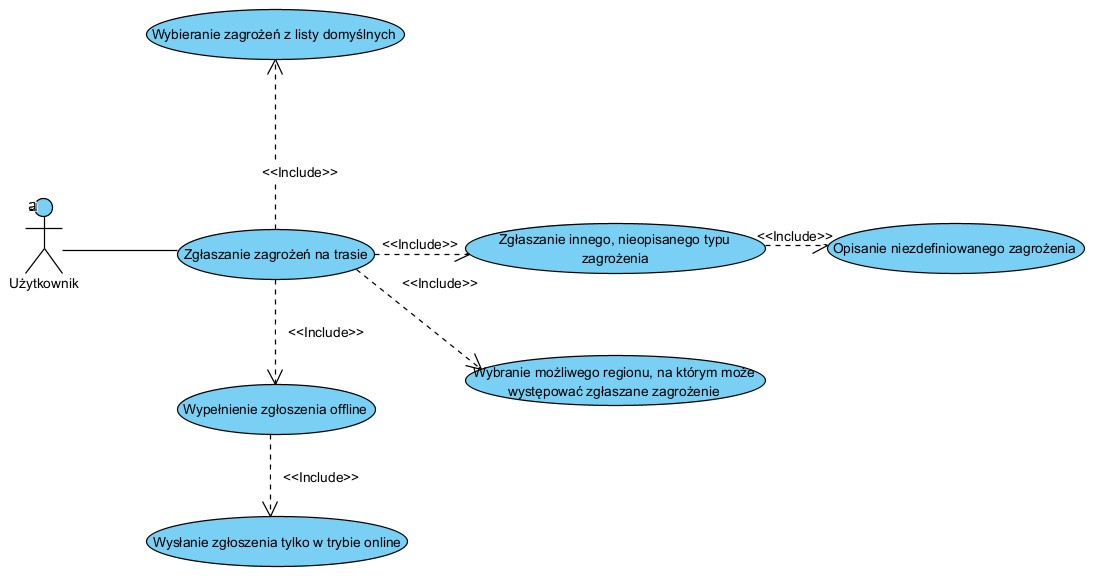
\includegraphics[width=\linewidth]{img/diagramy/UC/UCzagrozenie.jpg}}
        \caption{Diagram przypadku użycia: zgłaszanie zagrożeń.}
        \label{ucd:zagrozenia}
    \end{figure}
    Zgłaszanie zagrożeń oraz utrudnień występujących na szlaku (rys. \ref{ucd:zagrozenia}) pomaga wszystkim turystom bezpiecznie przejść całą zaplanowaną przez nich trasę. Występujące zagrożenie może zgłosić każdy z dostępem do internetu, lecz formularz zgłoszeniowy można wypełnić również w trybie offline. Zapisany i wypełniony formularz zostanie wysłany do zatwierdzenia, gdy urządzenie użytkownika uzyska dostęp do internetu. Zgłoszone zagrożenie posiada także przypisany region obowiązywania, tj. okolice lokalizacji użytkownika w momencie wypełnienia zgłoszenia. Użytkownik może wybrać typ zagrożenia z gotowej listy lub własnoręcznie opisać zdarzenie.

    \setlength{\fboxrule}{0.5pt}
    \begin{figure}[H]
        \centering
        \fbox{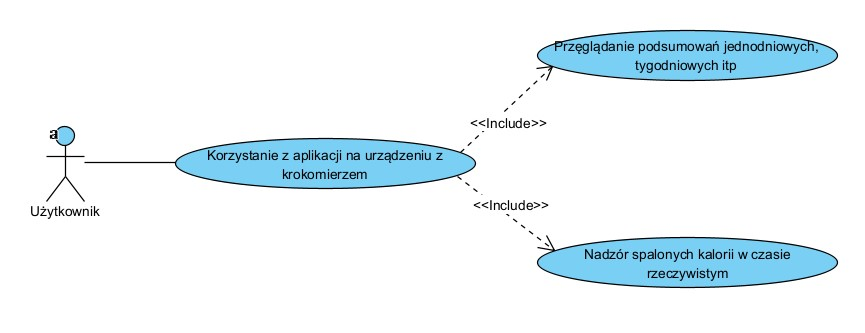
\includegraphics[width=\linewidth]{img/diagramy/UC/UCkrokomierz.jpg}}
        \caption{Diagram przypadku użycia: użycie krokomierza}
        \label{ucd:krokomierz}
    \end{figure}
    
    
    \subsection{Scenariusze}
    Scenariusze pozwalają rozpatrzeć dokładnie konkretne użycia danych funkcji oraz ich przebiegi alternatywne i sytuacje wyjątkowe. Poniższe wybrane scenariusze opisują kolejno: zgłoszenie zagrożenia przez użytkownika, wyznaczanie trasy, wysyłanie przez administratora powiadomienia o zagrożeniu do użytkowników oraz wyłączanie szlaku z użycia przez administratora.
    \subsection*{Scenariusz 1: Zgłaszanie zagrożeń}
    \noindent
    \textbf{S1.1 Opis} \par
    Scenariusz opisujący zgłaszanie przez użytkownika zagrożeń występujących na danej trasie w celu poinformowania innych o utrudnieniach przez aplikację mobilną. \\
    \textbf{S1.2. Aktorzy} \par
    Klient/użytkownik \\
    \textbf{S1.3. Warunki początkowe} \par
    Użytkownik jest zalogowany na aplikację i ma wyznaczoną trasę do przejścia. \\
    \textbf{S1.4. Warunki końcowe} \par
    System przesyła ogłoszenie o zagrożeniu do weryfikacji administratorowi. \\
    \textbf{S1.5. Przebieg główny} 
    \begin{enumerate}
        \item Użytkownik wybiera opcję zgłoszenia zagrożenia.
        \item System wyświetla listę z przykładowymi zagrożeniami.
        \item Użytkownik wybiera rodzaj zagrożenia z listy.
        \item System wyświetla zgłoszenie z obecną lokalizacją użytkownika.
        \item Użytkownik zatwierdza zagrożenie.
    \end{enumerate}
    \textbf{S1.6. Przebieg alternatywny}\par 
    \begin{enumerate}
        \item []PA 3.1 Użytkownik dodaje własny opis kategorii zagrożenia.
             \begin{enumerate}
                \item Użytkownik odpowiada na pytania w celu zidentyfikowania zagrożenia.
                \item Powrót do punktu 4 przebiegu głównego.
            \end{enumerate}
        \item [] PA 5.1 Użytkownik edytuje zgłoszenie.
            \begin{enumerate}
                 \item Użytkownik odpowiada na pytania w celu zidentyfikowania zagrożenia.
                 \item Powrót do punktu 4 przebiegu głównego.
            \end{enumerate}
    \end{enumerate}
    \textbf{S1.7. Sytuacje wyjątkowe} \par
    \begin{enumerate}
        \item[] SW 1. System nie może zlokalizować użytkownika.
           \begin{enumerate}
                \item  System wyświetla komunikat o błędzie.
            \end{enumerate}
    \end{enumerate}
    \textbf{S1.8. Wymagania niefunkcjonalne} \par
    Takie same jak do systemu ułatwiającego poruszanie się po górach \\
    \textbf{S1.9. Uwagi i pytania otwarte} \par
    Brak

    \subsection*{Scenariusz 2: Wyznaczanie trasy}
    \noindent
    \textbf{S2.1 Opis} \par
    Scenariusz opisujący wyznaczenie najlepszej trasy dla użytkownika. \\
    \textbf{S2.2 Aktorzy} \par
    Klient/użytkownik \\
    \textbf{S2.3 Warunki początkowe} \par
    Użytkownik jest zalogowany do aplikacji. \\
    \textbf{S2.4 Warunki końcowe} \par
    System wyświetla wybraną przez użytkownika trasę zaznaczoną na mapie. \\
    \textbf{S2.5 Przebieg główny}
    \begin{enumerate}
        \item Użytkownik wybiera opcję wyznaczania trasy.
        \item Użytkownik podaje cel wędrówki.
        \item System pokazuje dostępne szlaki.
        \item Użytkownik wybiera najlepszą dla niego trasę.
        \item System wyświetla informacje o dystansie oraz planowanym czasie wędrówki.
        \item Użytkownik zatwierdza wybraną trasę.
    \end{enumerate}
    \textbf{S2.6 Przebieg alternatywny}
    \begin{enumerate}
        \item[] PA 6.1 Użytkownik modyfikuje trasę, dodając przystanki na trasie.
        \begin{enumerate}
            \item Użytkownik dodaje nowy cel na trasie.
            \item Powrót do punktu 5 przebiegu głównego.
        \end{enumerate}
    \end{enumerate}
    \textbf{S2.7 Sytuacje wyjątkowe} \par
    \begin{enumerate}
        \item []SW 1. System nie może znaleźć dostępnej trasy dla użytkownika.
        \begin{enumerate}
            \item System wyświetla komunikat o błędzie.
        \end{enumerate}
    \end{enumerate}
    \textbf{S2.8. Wymagania niefunkcjonalne} \par
    Takie same jak do systemu ułatwiającego poruszanie się po górach. \\
    \textbf{S2.9. Uwagi i pytania otwarte} \par
    Brak 

    \subsection*{Scenariusz 3: Wysyłanie powiadomień do użytkowników w obrębie konkretnego regionu o miejscowym zagrożeniu bądź utrudnieniach.} 
    \noindent
    \textbf{S3.1.Opis} \par
    Scenariusz opisujący wysyłanie przez administratora powiadomień do użytkowników znajdujących się w obrębie danego regionu o miejscowym zagrożeniu. \\
    \textbf{S3.2. Aktorzy} \par
    Administrator \\
    \textbf{S3.3. Warunki początkowe} \par
    Administrator jest zalogowany na aplikację i jest połączony z internetem. \\
    \textbf{S3.4. Warunki końcowe} \par
    System wysyła powiadomienie o zagrożeniu do wszystkich użytkowników, którzy znajdują się w podanym przez administratora regionie. \\
    \textbf{S3.5. Przebieg główny} \par
    \begin{enumerate}
        \item  Administrator wybiera opcję wysłania powiadomienia do konkretnego regionu.
        \item System wyświetla listę z gotowymi, przykładowymi powiadomieniami.
        \item Administrator wybiera szablon i uzupełnia go o niezbędne informacje.
        \item Administrator wybiera region, w którym może występować zagrożenie.
        \item System wyświetla pełne powiadomienie ze wszystkimi szczegółami i czeka na potwierdzenie.
        \item Administrator zatwierdza powiadomienie.
    \end{enumerate}
    \textbf{S3.6. Przebieg alternatywny} \par
    \begin{itemize}
        \item []PA 3.1 Administrator pisze ręcznie całe powiadomienie.
        \begin{enumerate}
            \item System wyświetla pusty formularz.
            \item Administrator wpisuje treść powiadomienia ręcznie uwzględniając w nim wszystkie szczegóły.
            \item Powrót do punktu 4 przebiegu głównego.
        \end{enumerate}
    \end{itemize}
    \textbf{S3.7. Sytuacje wyjątkowe} \par
    \begin{itemize}
        \item []SW 1. Administrator traci połączenie z internetem w trakcie tworzenia treści powiadomienia.
        \begin{enumerate}
            \item System wyświetla informację o przełączeniu w tryb offline.
            \item System zapisuje wprowadzone do tej pory zmiany tak, aby po ponownym połączeniu z internetem powiadomienie było gotowe do wysłania.
        \end{enumerate}
    \end{itemize}
    \textbf{S3.8. Wymagania niefunkcjonalne} \par
    Takie same jak do systemu ułatwiającego poruszanie się po górach. \\
    \textbf{S3.9. Uwagi i pytania otwarte} \par
    Brak

    \subsection*{Scenariusz 4: Tymczasowe wyłączanie szlaków z użycia}
    \noindent
    \textbf{S4.1.Opis} \par
    Scenariusz opisujący tymczasowe wyłączanie szlaków z użycia przez administratora ze względu na prowadzone na nim prace konserwacyjne bądź inne, długotrwałe trudnienia. \\
    \textbf{S4.2. Aktorzy} \par
    Administrator \\
    \textbf{S4.3. Warunki początkowe} \par
    Administrator jest zalogowany na aplikację i jest połączony z internetem. \\
    \textbf{S4.4. Warunki końcowe} \par
    System wyszarza dany szlak na wszystkich mapach online i wyświetla komunikat o jego zamknięciu, gdy użytkownik chce go wybrać.\\
    \textbf{S4.5. Przebieg główny} \par
    \begin{enumerate}
        \item Administrator wybiera szlak, który chce wyłączyć z użycia.
        \item System wyświetla krótki formularz.
        \item Administrator podaje do formularza komunikat, dlaczego szlak jest zamknięty i przewidywaną datę jego ponownego otwarcia.
        \item System wyświetla gotowy do zatwierdzenia komunikat o zamknięciu szlaku.
        \item Administrator zatwierdza komunikat.
    \end{enumerate}
    \textbf{S4.6. Przebieg alternatywny} \par
    \begin{itemize}
        \item []PA 3.1 Administrator wyłącza jedynie część szlaku z użycia.
        \begin{enumerate}
            \item Administrator wybiera punkt, od którego szlak ma być wyłączony.
            \item System wyświetla inne, niezamknięte szlaki niedaleko tego, który obecnie wyłącza administrator.
            \item Administrator ustala obejście zamkniętej części szlaku.
            \item Powrót do punktu 2 przebiegu głównego.
        \end{enumerate}
    \end{itemize}
    \textbf{S4.7. Sytuacje wyjątkowe} \par
    \begin{itemize}
        \item []SW 1. Administrator traci połączenie z internetem w trakcie tworzenia treści powiadomienia.
        \begin{enumerate}
            \item System wyświetla informację o przełączeniu w tryb offline.
            \item System zapisuje wprowadzone do tej pory zmiany tak, aby po ponownym połączeniu z internetem powiadomienie było gotowe do wysłania.
        \end{enumerate}
    \end{itemize}
    \textbf{S4.8. Wymagania niefunkcjonalne} \par
    Takie same jak do systemu ułatwiającego poruszanie się po górach. \\
    \textbf{S4.9. Uwagi i pytania otwarte} \par
    Brak

    \subsection{Diagram klas}
    Diagram klas jest świetnym sposobem na przedstawienie struktury systemu w modelach obiektowych przez ilustrację struktury klas i zależności między nimi.
    Ukazuje on klasy (typy) obiektów w programie, w odróżnieniu od diagramu obiektów, który pokazuje jedynie egzemplarze (instancje) obiektów i ich zależności istniejące w konkretnym momencie.

    Poniższy diagram klas (rys. \ref{klasy}) opisuje strukturę systemu aplikacji wspomagającej turystykę górską. Składa się z następujących klas: Osoba, Użytkownik, Administrator, Zgłoszenie, Powiadomienie, Lokalizacja, Atrakcja, Szlak. Klasy te są ze sobą powiązane asocjacjami i agregacjami oraz korzystają z siebie nawzajem. 
    
    \begin{figure}[H]
        \centering
        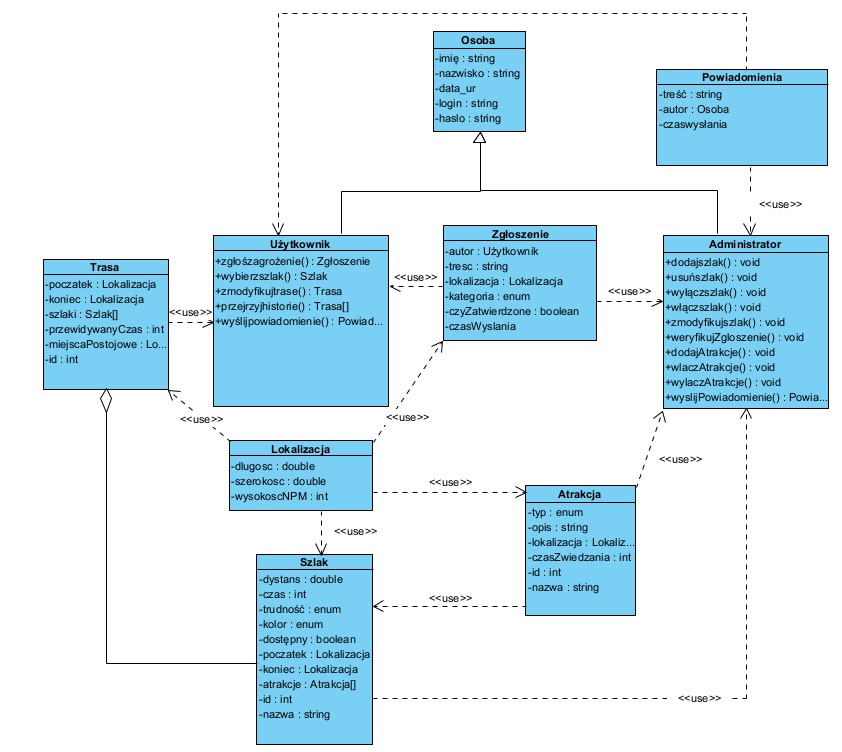
\includegraphics[width=\linewidth]{img/diagramy/klasyyy.jpg}
        \caption{Diagram klas}
        \label{klasy}
    \end{figure}
    \subsection*{Opis klas}
    \noindent
    \textbf{Klasa Osoba:}
    \begin{itemize}
        \item []Atrybuty:
        \begin{itemize}
            \item \textit{imię}: string - przechowuje imię danej osoby,
            \item \textit{nazwisko}: string - przechowuje nazwisko danej osoby,
            \item \textit{data\_ur} - przechowuje datę urodzenia danej osoby,
            \item \textit{login}: string  - przechowuje login użytkownika będący adresem e-mail danej osoby,
            \item \textit{haslo}: string - przechowuje szyfrowane hasło przypisane do konta danej osoby.
        \end{itemize}
    \end{itemize}
    \textbf{Klasa Użytkownik} \par
    Klasa ta dziedziczy po klasie Osoba przyjmując wszystkie jej atrybuty.
    \newpage
    \begin{itemize}
        \item []Funkcje:
        \begin{itemize}
            \item \textit{zgłośzagrożenie()} - zwraca nowo utworzony obiekt typu Zagrożenie z jego wszystkimi atrybutami,
            \item \textit{wybierzszlak()} - zwraca wybrany obiekt typu Szlak,
            \item \textit{zmodyfikujtrase()} - zwraca zmodyfikowany przez użytkownika obiekt Trasa,
            \item \textit{przejrzyjhistorie()} - zwraca listę Tras przebytych przez użytkownika,
            \item \textit{wyślijpowiadomienie()} - po zgłoszeniu Zagrożenia i zaakceptowaniu go przez Administratora wysyła Powiadomienie.
        \end{itemize}
    \end{itemize}
    \textbf{Klasa Administrator} \par
    Klasa ta dziedziczy po klasie Osoba przyjmując wszystkie jej atrybuty.
    \begin{itemize}
        \item []Funkcje:
        \begin{itemize}
            \item \textit{dodajszlak()} - funkcja void, tworzy nowy szlak i dodaje go do bazy danych,
            \item \textit{usuńszlak()} - funkcja void, usuwa wybrany szlak z bazy danych,
            \item \textit{wyłączszlak()} - funkcja void, wyłącza tymczasowo wybrany Szlak z użycia,
            \item \textit{włączszlak()} - funkcja void, włącza ponownie wybrany, uprzednio wyłączony \\z użycia Szlak,
            \item \textit{zmodyfikujszlak()} - funkcja void, modyfikuje istniejący już Szlak według nowych wytycznych,
            \item \textit{weryfikujZgłoszenie()} - funkcja void, pozwala na zweryfikowanie poprawności Zgłoszenia; po weryfikacji zamienia Zgłoszenie w Powiadomienie,
            \item \textit{dodajAtrakcje()} - funkcja void, dodaje do bazy danych nową Atrakcję do bazy Atrakcji dostępnych dla turystów,
            \item \textit{wylaczAtrakcje()} - funkcja void, wyłącza tymczasowo wybraną Atrakcję z użycia,
            \item \textit{wlaczAtrakcje()} - funkcja void, włącza ponownie wybraną, uprzednio wyłączoną z użycia Atrakcję,
            \item \textit{wyślijPowiadomienie()} - zwraca nowo utworzone Powiadomienie, które nie musi przechodzić procesu weryfikacji.
        \end{itemize}
    \end{itemize}
    \textbf{Klasa Zgłoszenie} 
    \begin{itemize}
        \item []Atrybuty:
        \begin{itemize}
            \item \textit{autor}: Użytkownik - przechowuje autora zgłoszenia, którym jest Użytkownik,
            \item \textit{tresc}: string - przechowuje treść opisu zgłoszenia,
            \item \textit{lokalizacja}: Lokalizacja - przechowuje Lokalizację pobraną z modułu GPS użytkownika w momencie wypełniania Zgłoszenia lub Lokalizację wybraną z mapy,
            \item \textit{kategoria}: enum - przechowuje wybraną z listy kategorię Zgłoszenia,
            \item \textit{czyZatwierdzone}: boolean - przechowuje informację, czy Zgłoszenie zostało zatwierdzone przez Administratora,
            \item \textit{czasWyslania} - przechowuje informację o czasie wysłania zgłoszenia celem sortowania ich przy wyświetlaniu Administratorowi do zatwierdzenia (od najwcześniej zgłoszonego).
        \end{itemize}
    \end{itemize}
    \textbf{Klasa Powiadomienie} 
    \begin{itemize}
        \item []Atrybuty:
        \begin{itemize}
            \item \textit{treść}: string - przechowuje treść zgłoszenia automatycznie wygenerowaną bądź zmodyfikowaną przez Administratora,
            \item \textit{autor}: Osoba - przechowuje dane autora Powiadomienia, którym może być zarówno Użytkownik jak i Administrator,
            \item \textit{czaswysłania} - przechowuje datę i czas wysłania Powiadomienia.
        \end{itemize}
    \end{itemize}
    \textbf{Klasa Lokalizacja}
    \begin{itemize}
        \item []Atrybuty:
        \begin{itemize}
            \item \textit{dlugosc}: double - przechowuje długość geograficzną,
            \item \textit{szerokosc}: double - przechowuje szerokość geograficzną,
            \item \textit{wysokoscNPM}: int - przechowuje wysokość punktu nad poziomem morza.
        \end{itemize}
    \end{itemize}
    \textbf{Klasa Szlak}
    \begin{itemize}
        \item []Atrybuty:
        \begin{itemize}
            \item \textit{dystans}: double - przechowuje długość danego Szlaku od jego początku do końca,
            \item \textit{czas}; int - przechowuje przybliżony czas potrzebny na przejście danego Szlaku (w minutach),
            \item \textit{trudność}: enum - przechowuje poziom trudności danego Szlaku,
            \item \textit{kolor}: enum - przechowuje kolor danego Szlaku według wytycznych kartograficznych,
            \item \textit{dostępny}: boolean - przechowuje informację o dostępności Szlaku (czy jest wyłączony z użycia lub czy turyści mogą się po nim poruszać),
            \item \textit{poczatek}: Lokalizacja - przechowuje dane lokalizacyjne o początku Szlaku,
            \item \textit{koniec}: Lokalizacja - przechowuje dane lokalizacyjne o końcu Szlaku,
            \item \textit{atrakcje}: Atrakcja[] - przechowuje listę Atrakcji dostępnych na wybranym Szlaku,
            \item \textit{id}: int - przechowuje identyfikator Szlaku,
            \item \textit{nazwa}: string - przechowuje nazwę Szlaku.
        \end{itemize}
    \end{itemize}
    \textbf{Klasa Atrakcja}
    \begin{itemize}
        \item []Atrybuty:
        \begin{itemize}
            \item \textit{typ}: enum - przechowuje typ Atrakcji,
            \item \textit{opis}: string - przechowuje krótki opis Atrakcji,
            \item \textit{lokalizacja}: Lokalizacja - przechowuje Lokalizację danej Atrakcji,
            \item \textit{czasZwiedzania}: int - przechowuje przybliżony czas zwiedzania Atrakcji (w minutach),
            \item \textit{id}: int - przechowuje identyfikator Atrakcji,
            \item \textit{nazwa}: string - przechowuje nazwę Atrakcji.
        \end{itemize}
    \end{itemize}
    \textbf{Klasa Trasa}
    \begin{itemize}
        \item []Atrybuty:
        \begin{itemize}
            \item \textit{poczatek}: Lokalizacja - przechowuje początek Trasy,
            \item \textit{koniec}: Lokalizacja - przechowuje koniec Trasy,
            \item \textit{szlaki}: Szlak[] - przechowuje listę Szlaków, którymi trzeba przejść, aby zrealizować daną Trasę,
            \item \textit{przewidywanyCzas}: int - przechowuje przewidywany czas potrzebny na przejście danej Trasy od początku do końca,
            \item \textit{miejscaPostojowe}: Lokalizacja[] - przechowuje listę zaplanowanych miejsc postojowych,
            \item \textit{id}: int - przechowuje identyfikator Trasy.
        \end{itemize}
    \end{itemize}

     \subsection{Diagram ERD}
   Diagram ERD (Entity-Relationship Diagram) to graficzne przedstawienie modelu danych, które pokazuje związki między różnymi elementami systemu. ERD składa się z trzech głównych komponentów: encje - reprezentują obiekty lub pojęcia, które mają znaczenie \\w kontekście bazy danych, atrybuty - określają właściwości lub cechy encji oraz związki - pokazują, jak encje są ze sobą powiązane.

     \begin{figure}[H]
        \centering
        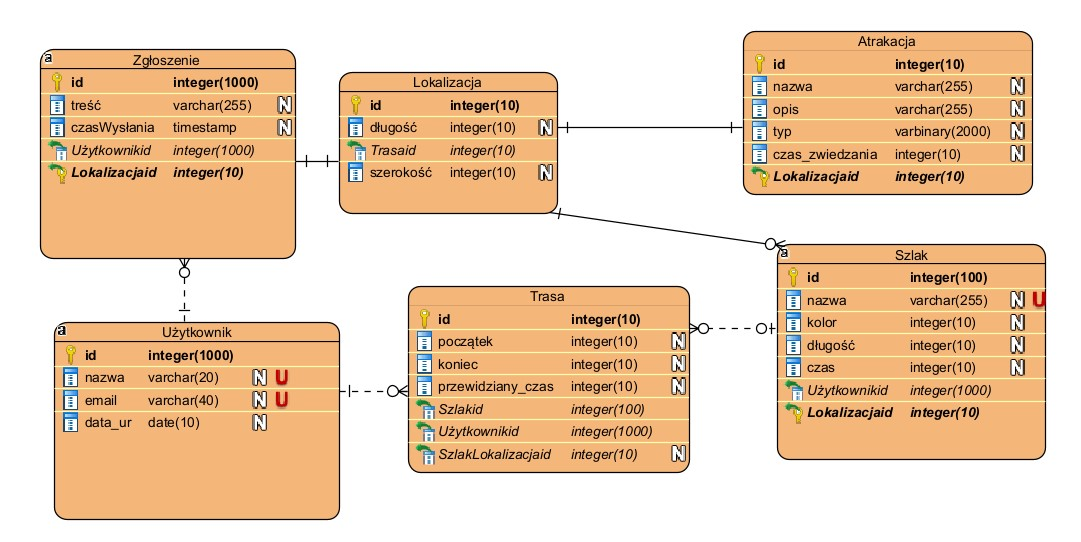
\includegraphics[width=\linewidth]{img/diagramy/erd.jpg}
        \caption{Diagram ERD.}
        \label{diagram:erd}
    \end{figure}
    Powyższy diagram prezentuje encje, atrybuty oraz powiązania istniejące w opisywanej aplikacji. \\
    \textbf{Encje i ich atrybuty}
    \begin{itemize}
        \item []Użytkownik
        \begin{itemize}
            \item \textit{id} typu integer jako klucz główny,
            \item \textit{nazwa} typu varchar (unikalna, niepusta),
            \item \textit{email} typu varchar (unikalny, niepusty),
            \item \textit{data\_ur} typu date (niepusta).
        \end{itemize}
        \item []Trasa
        \begin{itemize}
            \item \textit{id} typu integer jako klucz główny,
            \item \textit{początek} typu integer (niepusty),
            \item \textit{koniec} typu integer (niepusty),
            \item \textit{przewidziany\_czas} typu integer (niepusty),
            \item \textit{Szlakid} typu integer,
            \item \textit{Użytkownikid} typu integer,
            \item \textit{SzlakLokalizacjaid} typu integer (niepusta).
        \end{itemize}
        \item []Szlak
        \begin{itemize}
            \item \textit{id} typu integer (klucz główny),
            \item \textit{nazwa} typu varchar (unikalna, niepusta),
            \item \textit{kolor} typu integer (niepusty),
            \item \textit{długość} typu integer (niepusta),
            \item \textit{czas} typu integer (niepusty),
            \item \textit{Użytkownikid} typu integer,
            \item \textit{Lokalizacjaid} typu integer (klucz obcy).
        \end{itemize}
        \item []Zgłoszenie
        \begin{itemize}
            \item \textit{id} typu integer jako klucz główny,
            \item \textit{treść} typu varchar (niepusta),
            \item \textit{czasWysłania} typu timestamp (niepusty),
            \item \textit{Użytkownikid} typu integer,
            \item \textit{Lokalizacjaid} typu integer (klucz obcy).
        \end{itemize}
        \item []Lokalizacja
        \begin{itemize}
            \item \textit{id} typu integer jako klucz główny,
            \item \textit{długość} typu integer (niepusta),
            \item \textit{Trasaid} typu integer,
            \item \textit{szerokość} typu integer (niepusta).
        \end{itemize}
        \item []Atrakcja
        \begin{itemize}
            \item \textit{id} typu integer jako klucz główny,
            \item \textit{nazwa} typu varchar (niepusta),
            \item \textit{opis} typu varchar (niepusty),
            \item \textit{typ} typu varbinary (niepusty),
            \item \textit{czas\_zwiedzania} typu integer (niepusty),
            \item \textit{Lokalizacjaid} typu integer (klucz obcy),
        \end{itemize}
    \end{itemize}
    
    \noindent
    \textbf{Relacje}
    \begin{itemize}
        \item Zgłoszenie - Lokalizacja: jedno zgłoszenie musi mieć jedną lokalizację, ale z jednej lokalizacji można wysłać kilka zgłoszeń
        \item Użytkownik - Zgłoszenie: użytkownik może, ale nie musi wysłać wielu zgłoszeń, ale jedno zgłoszenie może być wysłane tylko przez jednego użytkownika,
        \item Użytkownik - Trasa: użytkownik może, ale nie musi stworzyć wiele tras, ale jedna trasa może być stworzona tylko przez jednego użytkownika,
        \item Trasa - Szlak: jeden szlak może, ale nie musi być zawarty w wielu trasach, a jedna trasa może przebiegać przez tylko jeden szlak,
        \item Lokalizacja - Szlak: jeden szlak zbudowany jest z wielu lokalizacji, ale jedna lokalizacja może występować tylko na jednym szlaku,
        \item Lokalizacja - Atrakcja: w jednej lokalizacji może występować tylko jedna atrakcja, \\a jedna atrakcja ma jedną lokalizację.
    \end{itemize}

    \subsection{Projekt interfejsu graficznego}
    Interfejs użytkownika jest kluczowym elementem doświadczenia użytkownika, wpływającym na to, jak użytkownicy postrzegają i korzystają z aplikacji. Dobrze zaprojektowany interfejs sprawia, że aplikacja jest intuicyjna, łatwa w użyciu i atrakcyjna wizualnie, co zwiększa satysfakcję użytkowników i ich efektywność.

    Poniżej ukazane są poglądowe interfejsy użytkownika zarówno dla zwykłego podróżnika, jak i administratora.
    
    \subsection*{Użytkownik}
    Użytkownik aplikacji ma dostęp do takich widoków jak: logowanie, rejestracja, widok główny zawierający mapę, profil użytkownika, historię przebytych tras, wybór trasy, telefony alarmowe oraz zgłoszenie zagrożenia. \\
    \\
    \textbf{Rejestracja} 
     \begin{figure}[H]
        \centering
        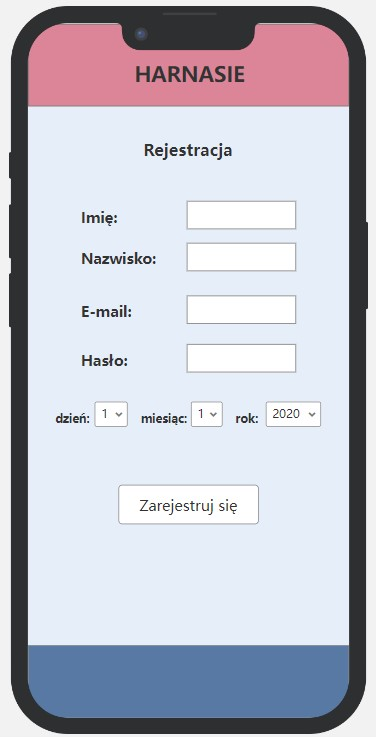
\includegraphics[scale=0.5]{img/interfejsy/if_rejestracja.jpg}
        \caption{Interfejs użytkownika: rejestracja.}
        \label{interfejs:rejestracja}
    \end{figure}
    Widok na rys.\ref{interfejs:rejestracja} zawiera formularz rejestracyjny, który pobiera od użytkownika następujące dane: imię, nazwisko, adres e-mail używany później jako login, hasło oraz datę urodzenia. Poniżej formularza znajduje się przycisk "Zarejestruj się", który dodaje użytkownika do bazy danych. Kliknięcie przycisku powoduje wyświetlenie powiadomienia o utworzeniu konta oraz przejście na ekran główny aplikacji(rys. \ref{interfejs:glowny}). \\
    \\
    \textbf{Logowanie} 
     \begin{figure}[H]
        \centering
        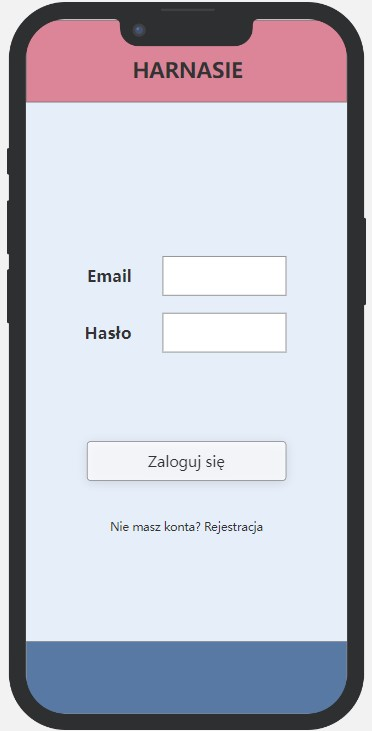
\includegraphics[scale=0.5]{img/interfejsy/if_loguj.jpg}
        \caption{Interfejs użytkownika: logowanie.}
        \label{interfejs:logowanie}
    \end{figure}
    Widok na rys.\ref{interfejs:logowanie} zawiera formularz logowania, który pobiera od użytkownika jego login oraz hasło. Poniżej pól do pobierania danych znajduje się przycisk "Zaloguj się", który przenosi użytkownika na ekran główny (rys. \ref{interfejs:glowny}). Oprócz tego widoczny jest odnośnik do formularza rejestracji (rys. \ref{interfejs:rejestracja}), jeśli użytkownik nie założył jeszcze konta w aplikacji. \\
    \newpage
    \textbf{Widok główny} 
     \begin{figure}[H]
        \centering
        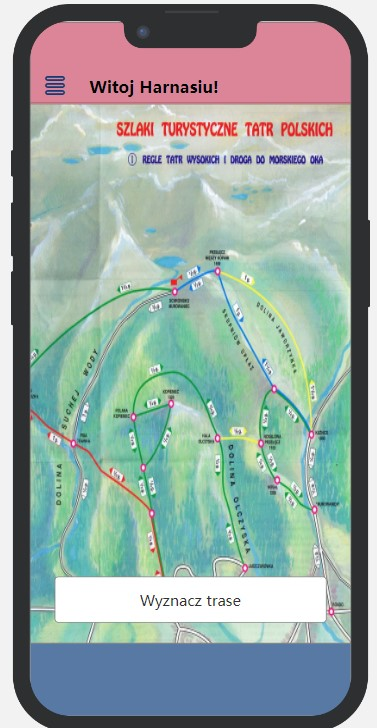
\includegraphics[scale=0.5]{img/interfejsy/if_główna.jpg}
        \caption{Interfejs użytkownika: widok główny.}
        \label{interfejs:glowny}
    \end{figure}
    Widok na rys.\ref{interfejs:glowny} zawiera interaktywną mapę, którą możemy przesuwać, przybliżać, oddalać. Na dole ekranu widoczny jest przycisk "Wyznacz trasę", przenoszący użytkownika do widoku z rys. \ref{interfejs:wyznacz}. W lewym górnym rogu widoczne jest zwijane menu aplikacji, które pozwala użytkownikowi przejście na wybrany widok aplikacji. \\
    \\
    \textbf{Menu rozwijane} 
     \begin{figure}[H]
        \centering
        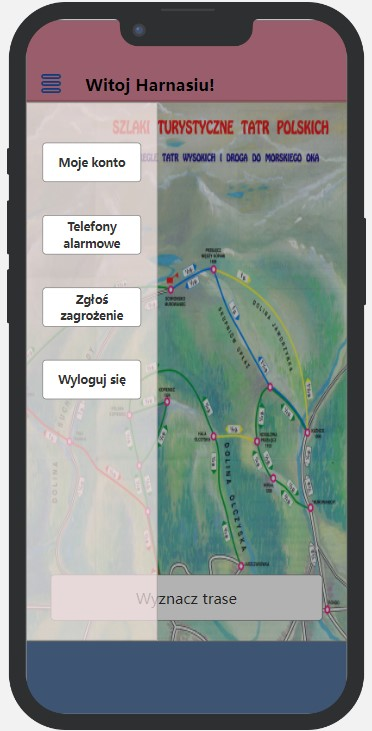
\includegraphics[scale=0.5]{img/interfejsy/if_menu.jpg}
        \caption{Interfejs użytkownika: menu rozwijane.}
        \label{interfejs:menu}
    \end{figure}
    Widok na rys.\ref{interfejs:menu} zawiera przyciski prowadzące do poszczególnych widoków aplikacji. Przycisk "Moje konto" przenosi użytkownika do widoku z rys. \ref{interfejs:konto}, przycisk "Telefony alarmowe" - do widoku z rys. \ref{interfejs:alarm}, "Zgłoś zagrożenie" - do widoku z rys. \ref{interfejs:zglos}, a "Wyloguj się" - do ekranu logowania (rys. \ref{interfejs:logowanie}). Menu rozwijane widoczne jest we wszystkich widokach aplikacji z wyłączeniem ekranu logowania (rys. \ref{interfejs:logowanie}) oraz rejestracji (rys. \ref{interfejs:rejestracja}). \\
    \\
    \textbf{Moje konto} 
    \begin{figure}[H]
        \centering
        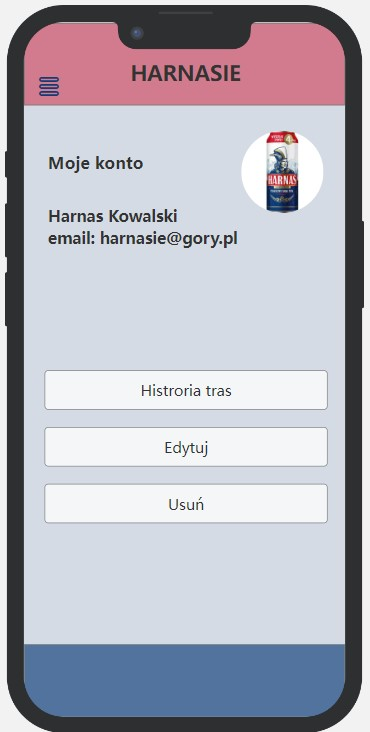
\includegraphics[scale=0.5]{img/interfejsy/if_konto.jpg}
        \caption{Interfejs użytkownika: moje konto.}
        \label{interfejs:konto}
    \end{figure}
    Widok na rys \ref{interfejs:konto} zawiera wypisane dane użytkownika, jego zdjęcie profilowe oraz przyciski pozwalające na przejrzenie historii wędrówek, edycję danych oraz usunięcie konta. \\W przypadku wybrania przycisku "Historia tras" użytkownik przenoszony jest do kolejnego, osobnego widoku (rys. \ref{interfejs:historia}). \\
    \\
    \textbf{Historia tras}
    \begin{figure}[H]
        \centering
        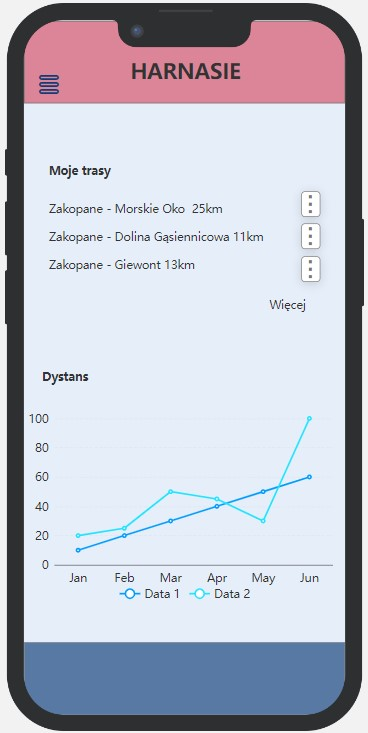
\includegraphics[scale=0.5]{img/interfejsy/if_historia.jpg}
        \caption{Interfejs użytkownika: historia przebytych tras.}
        \label{interfejs:historia}
    \end{figure}
   Widok na rys. \ref{interfejs:historia} zawiera historię przebytych przez użytkownika tras. Szczegóły każdej trasy użytkownik może zobaczyć klikając przycisk z trzema kropkami obok wybranej trasy. Poniżej wypisanych tras znajduje się także wykres, na którym użytkownik może zobaczyć wstępne, graficzne podsumowanie ostatnich wycieczek. \\
   \\
   \textbf{Wyznaczanie trasy}
    \begin{figure}[H]
        \centering
        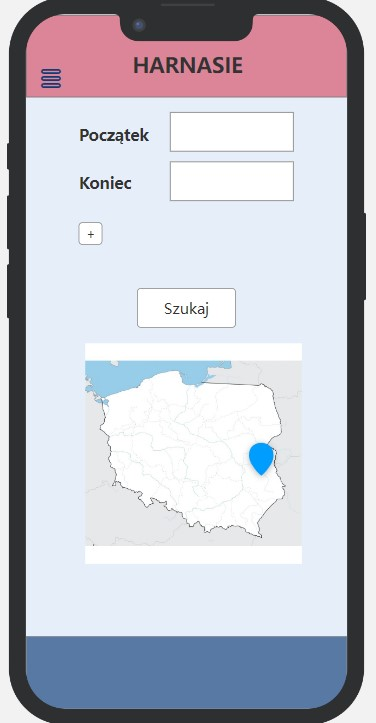
\includegraphics[scale=0.5]{img/interfejsy/if_wyznacz.jpg}
        \caption{Interfejs użytkownika: wyznaczanie trasy.}
        \label{interfejs:wyznacz}
    \end{figure}
   Widok na rys. \ref{interfejs:wyznacz} zawiera pola do wpisania początku i końca trasy, jaką użytkownik chce przejść. Pod nimi znajduje się przycisk "+", który pozwala na dodanie punktu postojowego i doprecyzowanie najbardziej pożądanej trasy. Wprowadzone dane po kliknięciu "Szukaj" wprowadzane są na mapę jako punkty i na ich podstawie wyznaczana jest najlepsza trasa, którą widać pod wyżej wymienionymi kontrolkami. \\
   \newpage
   \noindent
   \textbf{Zgłaszanie zagrożenia}
    \begin{figure}[H]
        \centering
        \includegraphics[scale=0.5]{img/interfejsy/if_zgłoszenie.jpg}
        \caption{Interfejs użytkownika: zgłoszenie zagrożenia.}
        \label{interfejs:zglos}
    \end{figure}
   Widok na rys. \ref{interfejs:zglos} zawiera listę rozwijaną typów zagrożeń, w tym możliwą opcją "inne", jeżeli dane zagrożenie nie zdarzyło się do tej pory. Każde zagrożenie można opisać w polu tekstowym poniżej. Po kliknięciu przycisku "Potwierdź" pojawia się powiadomienie o potwierdzeniu przesłania zgłoszenia do administratora, który zgłoszenie musi zatwierdzić (widok na rys. \ref{interfejs:zatwierdz}) \\
   \\
   \textbf{Telefony alarmowe}
    \begin{figure}[H]
        \centering
        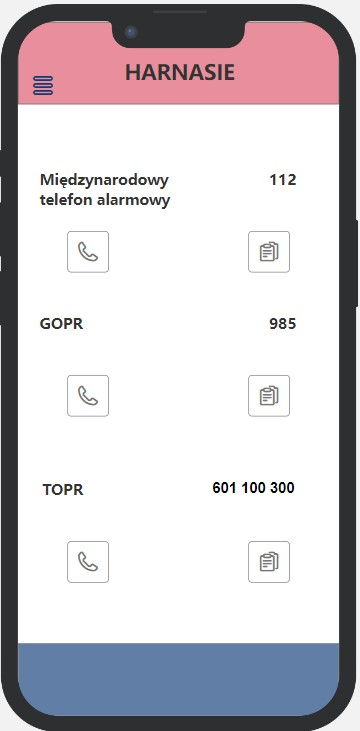
\includegraphics[scale=0.5]{img/interfejsy/if_alarmm.jpg}
        \caption{Interfejs użytkownika: telefony alarmowe.}
        \label{interfejs:alarm}
    \end{figure}
   Widok na rys. \ref{interfejs:alarm} zawiera wypisane ogólnopolskie telefony alarmowe, jak i numer na Górskie Ochotnicze Pogotowie Ratunkowe. Każdy numer można skopiować lub wybrać \\i zadzwonić na niego bezpośrednio z poziomu aplikacji.

    \subsection*{Administrator}
    Administrator aplikacji jest jednostką bardzo istotną dla poprawnego działania całej aplikacji. Po zalogowaniu na konto administratora (rys. \ref{interfejs:logowanie}) dostępne są następujące widoki: ekran główny, zatwierdzanie zgłoszeń przesłanych przez użytkowników, zarządzanie szlakami, zarządzanie atrakcjami, wysyłanie powiadomień oraz sekcja poświęcona GOPR.\\
    \\
    \textbf{Ekran główny}
     \begin{figure}[H]
        \centering
        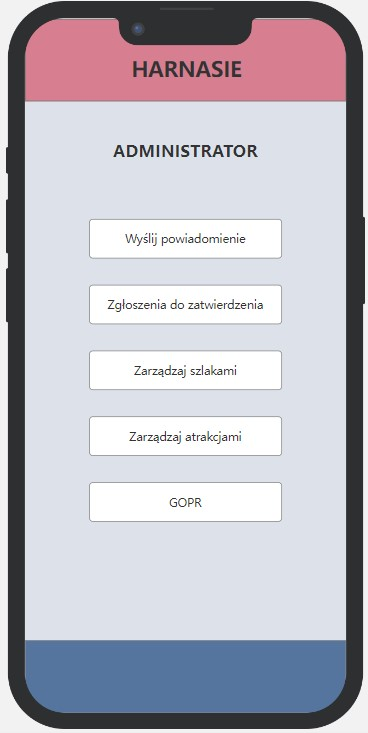
\includegraphics[scale=0.5]{img/interfejsy/if_admin.jpg}
        \caption{Interfejs użytkownika: ekran główny administratora.}
        \label{interfejs:admin}
    \end{figure}
   Widok na rys. \ref{interfejs:admin} zawiera kilka przycisków wspomagających nawigację po aplikacji. Dzięki tym przyciskom może przenieść się do ekranów: wyślij powiadomienie, zgłoszenia do zatwierdzenia, zarządzaj szlakami, zarządzaj atrakcjami oraz GOPR. Przyciski są odpowiednio nazwane, aby nie było wątpliwości, na jaki ekran użytkownik za chwilę zostanie przeniesiony. 
   \newpage
   \noindent
   \textbf{Zatwierdź zgłoszenia}
     \begin{figure}[H]
        \centering
        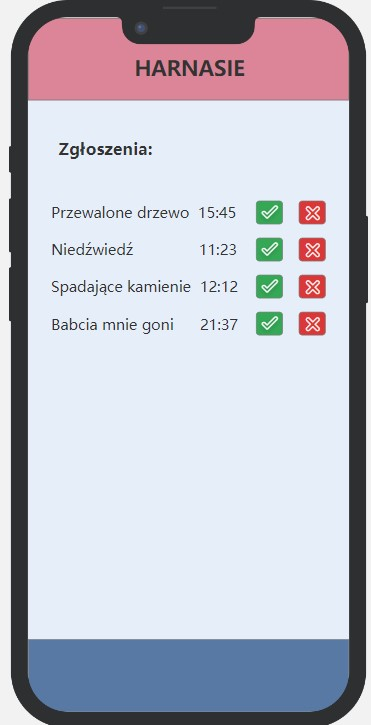
\includegraphics[scale=0.5]{img/interfejsy/if_zatwierdz.jpg}
        \caption{Interfejs użytkownika: zatwierdzanie zgłoszeń przesłanych przez użytkowników.}
        \label{interfejs:zatwierdz}
    \end{figure}
   Widok na rys. \ref{interfejs:zatwierdz} zawiera listę zgłoszonych, nierozpatrzonych jeszcze zgłoszeń użytkowników. Każdy element listy zawiera typ zgłoszenia, datę wysłania zgłoszenia oraz przyciski do akceptacji bądź odrzucenia konkretnego zgłoszenia. \\
   \\
   \textbf{Zarządzanie szlakami}
     \begin{figure}[H]
        \centering
        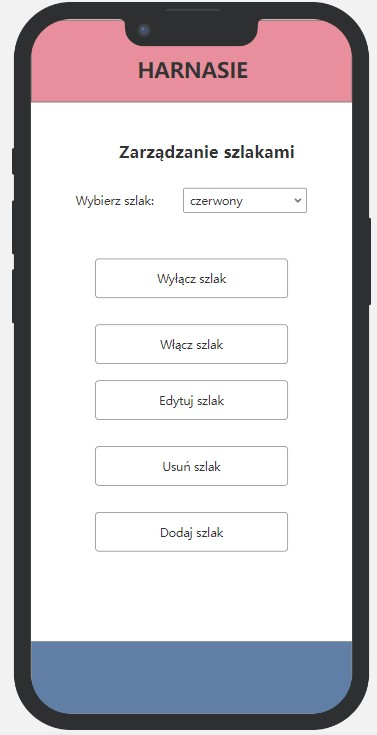
\includegraphics[scale=0.5]{img/interfejsy/if_zarzadzaj_szlaki.jpg}
        \caption{Interfejs użytkownika: zarządzanie szlakami.}
        \label{interfejs:szlaki}
    \end{figure}
   Widok na rys. \ref{interfejs:szlaki} zawiera listę rozwijaną szlaków dostępnych w bazie aplikacji. Administrator może z niej wybrać szlak, który wymaga modyfikacji a następnie wybrać jedną z dostępnych opcji edycji szlaku spośród: wyłącz szlak, włącz szlak, edytuj szlak oraz usuń szlak. Opcje włączenia i wyłączenia szlaku odnoszą się do tymczasowego blokowania szlaków z użycia ze względu na długotrwale występujące na nim utrudnienia, np. zasypany szlak po przejściu lawiny. Poniżej wszystkich przycisków związanych z modyfikacją istniejących już szlaków znajduje się jeszcze jeden, odpowiedzialny za  przejście do nowego widoku (rys. \ref{interfejs:dodaj}), gdzie możliwe jest dodanie nowego szlaku do bazy. \\
   \\
   \textbf{Dodaj szlak}
     \begin{figure}[H]
        \centering
        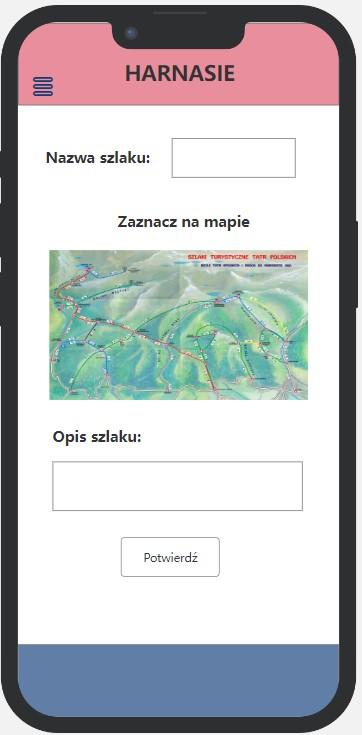
\includegraphics[scale=0.5]{img/interfejsy/if_nowy_szlak.jpg}
        \caption{Interfejs użytkownika: dodawanie nowego szlaku do bazy dostępnych szlaków.}
        \label{interfejs:dodaj}
    \end{figure}
   Widok na rys. \ref{interfejs:dodaj} zawiera kontrolki wspomagające wprowadzenie wszystkich niezbędnych informacji na temat nowego szlaku, który administrator chce utworzyć. Aby dodać nowy szlak należy podać jego nazwę, zaznaczyć jego przebieg na mapie oraz utworzyć krótki opis szlaku. Po kliknięciu przycisku "Potwierdź" wyświetla się powiadomienie informujące administratora o pomyślnym dodaniu szlaku do bazy.

   \subsection{Przegląd narzędzi implementacyjnych}
Dla prawidłowej i jak najskuteczniejszej pracy przygotowywanej aplikacji najważniejsze jest w procesie jej projektowania, aby dobrać optymalne narzędzia i technologie. W tym rozdziale skupiono się na krótkim omówieniu popularnych technologii programistycznych, które posiadają najbardziej potrzebne funkcje do prawidłowego działania systemu.

\subsection*{Usługi Firebase}
Dla prostej skalowalności całego projektu, a także usprawnienie połączeń między bazą danych a aplikacją oraz względne pozbycie się serwera aplikacji wielu programistów decyduje się na korzystanie z usług oferowanych przez Firebase \cite{firebase}. Do obsługi bazy danych najczęściej wybieraną usługą jest Firebase Firestore \cite{firebase-book}. Jest to szybka \\i elastyczna baza danych NoSQL, która działa w infrastrukturze Google Cloud i synchronizuje dane pomiędzy różnymi platformami.\par
Do usprawnienia logowania i autoryzacji w aplikacji często wykorzystuje się usługę Firebase Authentication \cite{fireauth} pozwalającą na sprawdzanie tożsamości użytkowników \\i personalizowanie treści wyświetlanych na urządzeniach klientów. Authentication obsługuje uwierzytelnianie przy użyciu haseł, numerów telefonów, a także kont na platformach mediów społecznościowych, takich jak Google, Facebook, Twitter i innych kanałów.\par
Przechowywanie plików w chmurze często jest potrzebne do sprawnej synchronizacji danych pomiędzy urządzeniami, kontami, jak i platformami. Firebase również tym razem wychodzi programistom na przeciw, udostępniając usługę Storage. Jest to wydajna, prosta \\w obsłudze i niedroga usługa pamięci masowej opracowana z myślą o skali Google.

\subsection*{Google Maps Platform}
Po dogłębnym przeszukaniu rynku oferującego wiele API obsługujących mapy na platformę Android, Google Maps Platform \cite{gmapsand} okazała się najbardziej odpowiednia. Jest to jedno z wielu usprawnień oferowanych przez Google przez dostęp do ich Google Clouds Platform. Dzięki temu wszelkie inne API z kategorii takich jak: obliczenia, przechowywanie i bazy danych, analiza danych, sztuczna inteligencja, sieci itp. są ze sobą zsynchronizowane, a do obsługiwania ich wszystkich wystarczy jedno konto, które przez pierwsze 90 dni jest darmowe i posiada 300USD przypisanych do portfela usługi. Po tym czasie użytkownik może zmienić typ swojego konta na płatne, wtedy środki pobierane są bezpośrednio z karty użytkownika za każde ponadplanowe użycie zasobów.
Aspekt płatności, choć może się wydawać odstraszający dla wielu, nie jest skomplikowany i pozwala na w pełni darmowy rozwój aplikacji, jednak przy komercjalizacji projektu darmowe zasoby mogą okazać się niewystarczające. \cite{gmapsogol}


\subsection*{Android Studio}
Najpopularniejsze IDE pozwalające na tworzenie aplikacji mobilnych na urządzenia \\z systemem Android \cite{androidstudio} \cite{android-studio-book}. Obsługuje język Java oraz Kotlin i zawiera wiele wbudowanych narzędzi ułatwiających tworzenie aplikacji na urządzenia mobilne. Posiada m.in. emulatory urządzeń, integrację z systemem kontroli wersji Git oraz narzędzia do profilowania wydajności aplikacji.

\subsection*{Język Java}
Java \cite{java} jest to wysokopoziomowy, obiektowy język programowania. Jego szeroki zakres użytku pozwala na tworzenie różnych aplikacji w zależności od potrzeby, m.in. aplikacji webowych, systemów biznesowych, aplikacji mobilnych (Android), a także można go wykorzystać w systemach wbudowanych i przetwarzaniu danych \cite{java-book}.
Dlaczego Java?
\begin{itemize}
    \item Obiektowość. Napisany kod można wykorzystywać wielokrotnie i dzielić go na moduły.
    \item Ogromny zasób gotowych bibliotek, które obsługują wszelakie funkcje.
    \item Aplikacje tworzone w Javie można uruchamiać na wszelkiego typu urządzeniach dzięki maszynie wirtualnej (JVM).
\end{itemize}

Aplikacja Harnasie umożliwia nam bezpieczne wędrówki po górach w rejonie Tatr Polskich. Dzięki opcji zgłaszaniu zagrożeń, które administrator akceptuje, poprawia się bezpieczeństwo wszystkich użytkowników. Wszyscy turyści korzystający z aplikacji zostaną powiadomieni o zagrożeniach miejscowych oraz otrzymają powiadomienie ogólne o komunikatach przekazywanych przez Tatrzańskie Ochotnicze Pogotowie Ratunkowe i Tatrzański Park Narodowy. Aplikacja śledzi również aktywność użytkownika oraz tworzy z niej przejrzysty wykres w interfejsie profilu. Zalogowany użytkownik może dzięki temu w prosty sposób zobaczyć swoje osiągnięcia oraz rozpowszechnić je znajomym, gdyż wszytskie dane zawierają się na jednym widoku. Harnasie posiada także funkcję wyznaczania trasy na mapie oraz możliwość wyboru sposobu nawigacji po niej. Użytkownik z dobrą orientacją w terenie może korzystać z trasy wyznaczonej w aplikacji, a dla osób, które wolą nawigację dostępną w Google Maps istnieje opcja otworzenia wyznaczonej trasy właśnie w tej aplikacji. Pozwala to wtedy na dokładne naprowadzanie po szlaku i zmniejsza ryzyko zagubienia się. Aplikacja zawiera także naniesione kolorami szlaki turystyczne na mapę, aby zapwenić przejrzystość \\i rozwiać wątpliwości o rodzaju szlaku. Często zdarza się, że idąc po wyznaczonym w górach szlaku, nawet na rozdrożu, ciężko zobaczyć oznaczenia kolorystyczne oznaczające długość szlaku. 


  